\section{Revisiting The Art of Computer
Programming}\label{revisiting-the-art-of-computer-programming}

\begin{frame}{Outline}

\begin{itemize}
\item
  Short presentation/introduction to Knuth and his perception of
  programming
\item
  Neural plasticity
\item
  Brain Imaging studies
\item
  examples: taxi drivers and musicians, WHY NOT SOFTWARE DEVELOPERS
\item
  one study, Siegmund et. al. 2014, ``reading code''
\end{itemize}

Donald Knuth (*10/01/1938) --------------------------

\begin{figure}
\centering
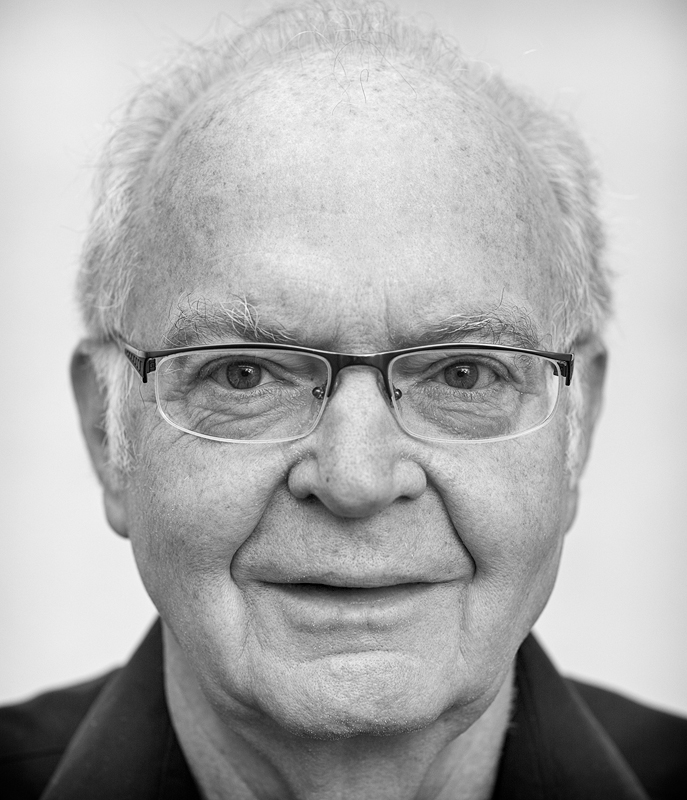
\includegraphics{./media/Knuth-A-small.jpg}
\caption{left}
\end{figure}

\begin{itemize}
\tightlist
\item
  Professor Emeritus at Stanford
\item
  Put the \textbf{Science} into Computer Science
\item
  Father of \(TeX\)
\item
  Featured thrice in XKCD
\end{itemize}

\begin{figure}
\centering
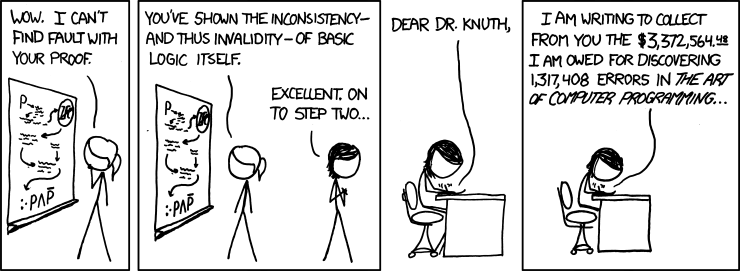
\includegraphics{./media/xkcd-applied_math.png}
\caption{}
\end{figure}

\begin{quote}
Everyday life is like programming, I guess. If you love something you
can put beauty into it. (Not verified, can't find reference)
\end{quote}

More on the relationship between art and programming for Knuth

\end{frame}

\begin{frame}{The Art of Computer Programming (TAOCP)}

\begin{quote}
The process of preparing programs for a digital computer is especially
attractive, not only because it can be economically and scientifically
rewarding, but also because it can be an \textbf{aesthetic experience
much like composing poetry or music}. {[}emphasis added{]} (The Art of
Computer Programming (1968), Vol. 1, v.)
\end{quote}

\end{frame}

\begin{frame}{Creativity and programming}

Software development is inherently creative and is influenced by fields
based in the aesthetics. Think about \textbf{Gang Of Four: Design
Patterns: Elements of Reusable Object-Oriented Software}

\begin{quote}
A design pattern is the re-usable form of a solution to a design
problem. The idea was introduced by the architect Christopher Alexander
and has been adapted for various other disciplines, most notably
computer science.
\end{quote}

\begin{quote}
Science is knowledge which we under- stand so welt that we can teach it
to a computer; and if we don't fully understand something, it is an art
to deal with it. (Knuth1974)
\end{quote}

\begin{quote}
The science without tile art is likely to be ineffective; the art
without tile scierce is certain to be inaccurate." (Knuth1974)
\end{quote}

\begin{quote}
When I speak about computer programming as an art, I am thinking
primarily of it as an art form, in an aesthetic sense. The chief" goal
of my work as educator and author is to help people learn how to write
beau- tiJM programs. (Knuth1974)
\end{quote}

\begin{quote}
Some programs are elegant, some are exquisite, some are sparkling. My
claim is that it is possible to write grand programs, treble programs,
truly magnificent ones! (Knuth1974) Neural plasticity -----------------
What does it mean to program and how does it influence you.
\end{quote}

Brain studies show how your work changes your brain.

\begin{itemize}
\item
  Recovery after impairment: Phineas Gage: Neuroscience's Most Famous
  Patient \includegraphics{./media/Phineas-Gage.png}
\item
  London tazi drivers
\item
  Musicians vs.~non-musicians
\item
  Practiced musical style shapes auditory skills
\item
  Tapping polyrhythms in music activates language areas
\end{itemize}

Ability for a region to be recruited in an otherwise unrelated task
through continued adaptation and practice.

``Borrowing'' processing power from a different region

\begin{quote}
``superior visuospatial cognitive performance in action video game
experts'' ``\ldots{}larger gray matter volume in the right posterior
parietal cortex in experts compared with non-experts''
\end{quote}

1 study which looks at cognitive processing for software developers

\begin{itemize}
\tightlist
\item
  Is something specific for this field.
\item
  computer programming is a study, a major part of this is learning to
  think in a specific way.
\end{itemize}

\textbf{Sub reddit discussing the Neuroscience of Programming:}
https://www.reddit.com/r/programming/comments/1ypetm/a\_programmers\_brain\_on\_code\_the\_neuroscience\_of/

http://www.thebioneer.com/hackers-brain-the-psychology-of-programming/

\begin{quote}
Besides a mathematical inclination, an exceptionally good mastery of
one's native tongue is the most vital asset of a competent programmer.
(Dijkstra)
\end{quote}

\begin{quote}
Experienced London taxi drivers have larger parahippocampal regions with
size correlated with years of experience. (Maguire2006)
\end{quote}

\begin{quote}
simple, focused, and energy-efficient action in the brain.
\end{quote}

\end{frame}

\begin{frame}[fragile]{Neuroscience of programming (Siegmund et. al.
2014)}

functional Magnetic Reasonance Imaging (fMRI) - measure brain activity
as a function of the level of oxygenated blood flow

Used fMRI to study how programmer's understand source code - simple
tasks

\begin{Shaded}
\begin{Highlighting}[]
\KeywordTok{public} \DataTypeTok{static} \DataTypeTok{void} \FunctionTok{main}\NormalTok{(}\BuiltInTok{String}\NormalTok{[] args)}
\NormalTok{\{}
    \BuiltInTok{String} \NormalTok{word = }\StringTok{"Hello"}\NormalTok{;}
    \BuiltInTok{String} \NormalTok{result = }\KeywordTok{new} \BuiltInTok{String}\NormalTok{();}

    \KeywordTok{for} \NormalTok{(}\DataTypeTok{int} \NormalTok{j = word.}\FunctionTok{length}\NormalTok{(); - }\DecValTok{1}\NormalTok{; j >=}\DecValTok{0}\NormalTok{; j--)}
        \NormalTok{result = result + word.}\FunctionTok{charAt}\NormalTok{(j);}

    \BuiltInTok{System}\NormalTok{.}\FunctionTok{out}\NormalTok{.}\FunctionTok{println}\NormalTok{(result);}
\NormalTok{\}}
\CommentTok{//  Source code for one comprehension task with expected output ‘olleH‘.}
\end{Highlighting}
\end{Shaded}

\begin{quote}
programming had less in common with mathematics and more in common with
language.
\end{quote}

Studies comparing subjects with and without a computer science
background.

\textbf{Christopher Parnin: http://www.chrisparnin.me}

\begin{itemize}
\tightlist
\item
  Can we finally provide a neurological basis for a programmer's flow
  (being in the zone)?
\item
  What will studying an expert programmer's brain reveal? How might
  years of programming experience manifest as changes in the brain?
\item
  Are there certain programming activities that should never be mixed
\end{itemize}

\end{frame}
